\section{Coarse-to-Fine Streaming Data Engine}\label{sec:data_pipe}

\begin{figure}[t]
    \centering
    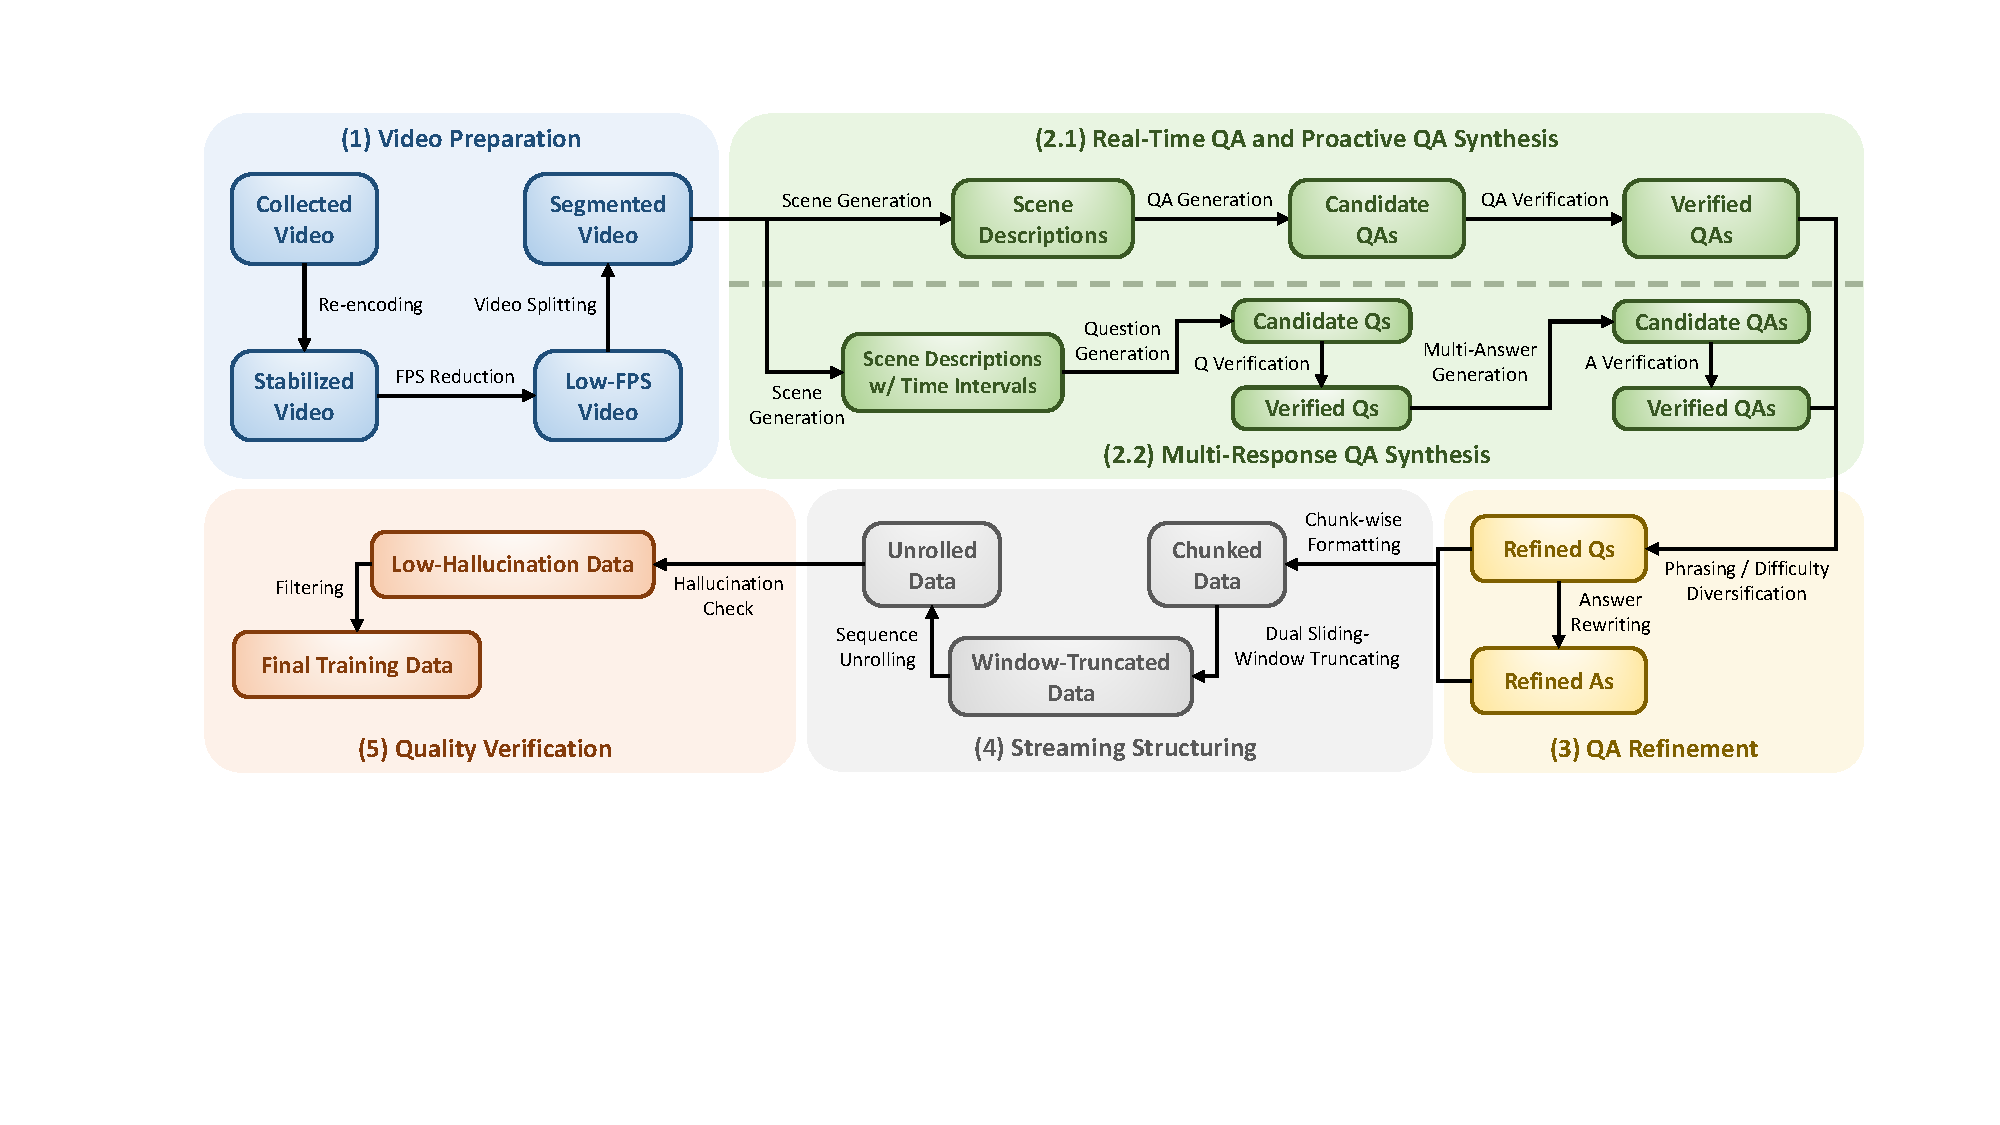
\includegraphics[width=\textwidth]{img/4_Data_pipeline_2.pdf}
    \caption{Overview of the Coarse-to-Fine Streaming Data Engine in AURA. The pipeline comprises five stages: (1) Video Preparation, (2) QA Synthesis, (3) QA Refinement, (4) Streaming Structuring, and (5) Quality Verification.}
    \label{fig:data_pipeline}
\end{figure}

Building on the QA categories defined above, we develop a coarse-to-fine data engine to generate streaming training data for Real-Time QA, Proactive QA, and Multi-Response QA. As illustrated in Figure~\ref{fig:data_pipeline}, the pipeline consists of five stages:  (1) \textbf{Video Preparation}, (2) \textbf{QA Synthesis}, (3) \textbf{QA Refinement}, (4) \textbf{Streaming Structuring}, and (5) \textbf{Quality Verification}.
This pipeline translates the interaction taxonomy into structured supervision, enabling the model to learn both when to respond and what to respond under different interaction patterns, thereby providing a strong data foundation for AURA.


\subsection{Video Preparation}
We collect high-quality videos from public internet sources covering a broad range of categories, including sports, vlogs, documentaries, encyclopedic content, TV shows, movies, courses, games, and animation. Then, each video is resampled to a fixed frame rate of 2 FPS to balance temporal coverage and computational cost, and re-encoded in H.264 format~\citep{wiegand2003overview} to improve codec consistency and decoding stability, while mitigating issues caused by corrupted or undecodable frames.

\subsection{QA Synthesis}
After obtaining standardized videos from the previous stage, we design two distinct pipelines to synthesize streaming QA. This separation is motivated by the different temporal structures of the QA types: Real-Time and Proactive QA require only a single response, whereas Multi-Response QA involves multiple valid answers to the same question at different time points. In the following, we describe each pipeline in detail.


The first pipeline focuses on Real-Time and Proactive QA. For each video, we first apply a multimodal large language model (MLLM) to perform scene segmentation and generate scene-level descriptions for each segment, thereby capturing the temporal progression of events throughout the video. Based on the video and its scene-level descriptions, the MLLM then produces candidate QA pairs with associated question and answer timestamps. For Real-Time QA, the question and answer share the same timestamp; for Proactive QA, the question timestamp precedes the answer timestamp. We then ask the MLLM to verify each candidate QA pair using only the video content up to the answer timestamp. For Real-Time QA, the MLLM checks whether the question is reasonable, whether the answer is correctly supported by the video content, and whether the timestamp is accurate. For Proactive QA, the MLLM further checks whether the question can be naturally raised at the question timestamp and whether sufficient information is available by the answer timestamp. Only QA pairs that pass the corresponding verification step are retained.


The second pipeline is designed for Multi-Response QA. For each video, we first apply an MLLM to perform scene segmentation and generate scene-level descriptions together with the corresponding time intervals for each scene. Then, for each video clip spanning a given time interval, we provide its scene description to the MLLM to generate candidate questions and their associated timestamps. Next, each candidate question is checked to determine whether it is reasonable and whether it can produce multiple valid answers at different timestamps within the video clip. Only the questions that satisfy both conditions are retained. For each retained question, we again prompt the MLLM with the corresponding video clip to generate multiple answers and their associated timestamps. Each generated answer is then verified to ensure that it can be correctly inferred at the specified timestamp and that it appropriately answers the question. Finally, the validated answers are retained to construct Multi-Response QA samples.





\subsection{QA Refinement}

We observe that QA samples generated in the QA Synthesis stage still exhibit limited diversity. In particular, Real-Time QA tends to exhibit limited diversity in difficulty levels, while Proactive QA and Multi-Response QA often show limited diversity in question phrasing. To better capture the diversity of difficulty levels and phrasings in real-world user queries, we design tailored refinement strategies for different QA types.

For Real-Time QA, we focus on enriching the diversity in difficulty levels. Specifically, for each original QA pair associated with a timestamp, we prompt the MLLM to generate four additional questions anchored at the same timestamp as the original question. These questions are designed to span progressively increasing levels of difficulty, from simple perceptual recognition to advanced understanding and reasoning. As a result, we obtain five candidate questions for each timestamp, including the original question and four augmented questions at different difficulty levels.
We then sample one question from these five candidates using a balanced sampling ratio. After the question is selected, we prompt the MLLM to generate an answer aligned with the sampled question based on the same video prefix, yielding the final refined QA pair.



For Proactive QA and Multi-Response QA, we focus on increasing the diversity in question phrasing by rewriting each question into different yet semantically equivalent forms. Specifically, we predefine a set of candidate templates for both Proactive and Multi-Response questions. For each question, we randomly select one template and use an LLM to generate a rewritten version accordingly. During this process, key entities, actions, and temporal references are kept unchanged to ensure consistency with both the original meaning and the video content. In this way, we enhance linguistic diversity without changing the core semantics of the original QA pairs.


\subsection{Streaming Structuring}
\label{sec:strm_struc}

Once timestamped QA annotations are obtained, this stage converts them into training samples that match the Interactive Video Stream Context Management mechanism through chunk-wise formatting and dual sliding-window truncating. In actual streaming inference, the model generates each response online based on the video window and the retained QA history available at that moment. Accordingly, during training, answers with different timestamps within the same continuous QA sequence should be paired with their corresponding video content and contextual history. We therefore unroll each sequence of continuous QA interactions from the same video into multiple training samples, each containing the interaction history up to one non-silent assistant message to be supervised, which we refer to as the target answer. For each sample, we use the timestamp of the target answer as the anchor for determining the time window. During training, we supervise only this target answer, while retaining the earlier QA interactions as contextual history (the specific supervision target is described in Section~\ref{silent-speech_balanced_loss}). This design helps bridge the gap between the necessary window truncation in long streaming contexts and the need for reliable supervision signals.


\subsection{Quality Verification}
\label{sec:quality_verify}





Since the previous stage reformats each sample within a truncated streaming context window, the retained video content and contextual history may become insufficient to support the target answer. Training on such samples may lead the model to generate content that is not grounded in the available visual input, thereby increasing the risk of hallucination. To address this issue, we introduce a dedicated Quality Verification stage.

For Real-Time QA, verification focuses on whether the target answer is supported by the relevant visual evidence available up to the response moment together with the retained QA history. The judge evaluates whether the answer is visually grounded, factually correct, temporally consistent, and free of hallucination. Only samples that satisfy these criteria are retained. For Proactive QA and Multi-Response QA, verification focuses on whether the target answer is temporally appropriate and whether its content is accurate and grounded in the retained video context and QA history. Samples are retained only when both criteria are satisfied. This stage filters out unreliable samples, helping ensure that the remaining data meet quality standards.












\subsection{Additional Details}



Beyond the five-stage pipeline, we introduce two practical designs to better align the training data with real-world streaming interactions. First, for Proactive QA and Multi-Response QA, we insert a short acknowledgment immediately after each user query to indicate that the request has been received and that an actual response will follow later, thereby improving the user experience. Second, because real streaming sessions often involve multiple interaction patterns within a single video, we combine Real-Time QA, Proactive QA, and Multi-Response QA generated from the same source video into mixed interaction sequences according to their timestamps. This design helps the model handle interleaved QA patterns more effectively in realistic streaming scenarios.























































